\documentclass[11pt]{article}

\usepackage{a4wide}
\usepackage[czech]{babel} 
\usepackage[utf8]{inputenc}
\usepackage[T1]{fontenc}
\usepackage{graphicx}
\usepackage{charter}
\usepackage{float}

\newcommand\uv[1]{\quotedblbase #1\textquotedblleft}%

\floatstyle{ruled}
\newfloat{vystup}{H}{lop}
\floatname{vystup}{Výstup}

\begin{document}
\author{David Marek}
\title{Uživatelská dokumentace programu Diff}
\date{}
\maketitle{}

\newpage{}

\section{Úvod}

\paragraph{}
Unixový program {\tt diff} slouží k zobrazení rozdílů mezi dvěma soubory. 
Pro dva soubory řekne, které řádky byly přidány nebo naopak odebrány.
Program diff je proslulý na unixových systémech. Společně s 
programem {\tt patch} se staly programy, které napomohly open source vývoji.
Tento program je grafickou verzí programu diff. V přívětivém rozhraní
zobrazuje rozdíly mezi soubory a barevně je i zvýrazní. Samozřejmě umožňuje
i stejný výstup jako unixová utilita stejného názvu.
Tato dokumentace slouží k seznámení uživatele s možnostmi programu.

\section{Rozhraní}

\subsection{Hlavní okno}

\paragraph{}
První, co uživatel po spuštění programu vidí je hlavní okno, kde se 
zobrazují oba porovnávané soubory dohromady s barevně vyznačenými změnami.
\\

\begin{figure}[H]
\centering
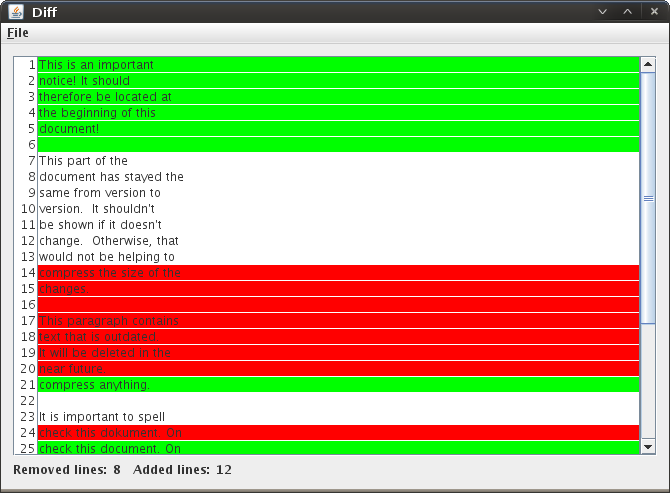
\includegraphics[scale=0.6]{scr1.png}
\caption{Hlavní okno se zobrazeným diffem.}
\end{figure}

\paragraph{}
Bez podbarvení jsou řádky společné staré i nové verzi. Zeleně podbarvené 
jsou řádky nově přidané a červeně podbarvené jsou odebrané řádky. Ve spodní
části okna jsou statistické informace o souboru, počet odebraných a 
přidaných řádků.

\begin{figure}[H]
\centering
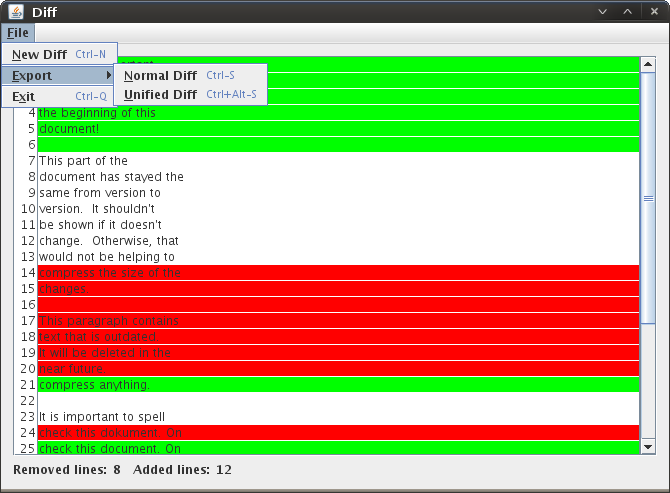
\includegraphics[scale=0.6]{scr2.png}
\caption{Menu aplikace.}
\end{figure}

\paragraph{}
Nejdřív se ovšem musí vstupní soubory vybrat, k tomu slouží položka 
{\em New Diff} v menu. Otevře dialog pro výběr souborů.

\subsection{Dialog pro porovnání souborů}

\paragraph{}
Uživatel musí vybrat dva soubory, které se budou porovnávat, první soubor je
původní, druhý je ten \uv{novější}.

\begin{figure}[H]
\centering
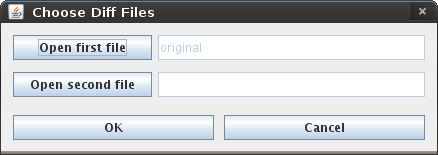
\includegraphics[scale=0.6]{scr3.png}
\caption{Výběr souborů.}
\end{figure}

\section{Export}

\paragraph{}
Kromě grafického zobrazení je možné diff i exportovat do souboru. Program 
nabízí dva různé formáty. První z nich je \emph{normální diff}. To je 
standardní výstup unixového programu {\tt diff}. Změny jsou rozděleny do bloků,
na začátku každého bloku jsou informace o tom, na kterém řádku změny začínají,
kolik řádků je změněno, zda-li byli řádky přidány, odebrány nebo změněny(a,d,c)
a nakonec je umístění a počet těchto řádku v novém souboru.

Druhá možnost je \emph{unified diff}. Od normalního se liší formátem, řádky
jsou označeny symboly + a --, ale navíc jsou přidány i tzv. kontextové
řádky okolo změn pro lepší orientaci. A také je na začátku přidána hlavička
obsahující názvy souborů, cestu k nim a také timestamp.

\begin{vystup}
\begin{verbatim}
0a1,6
> This is an important
> notice! It should
> therefore be located at
> the beginning of this
> document!
> 
8,14c14
< compress the size of the
< changes.
< 
< This paragraph contains
< text that is outdated.
< It will be deleted in the
< near future.
---
> compress anything.
17c17
< check this dokument. On
---
> check this document. On
24a25,28
> 
> This paragraph contains
> important new additions
> to this document.
\end{verbatim}
\caption{Normální diff.}
\end{vystup}

\begin{vystup}
\begin{verbatim}
--- /home/david/programovani/Diff/test/test_w/original	1235686522000
+++ /home/david/programovani/Diff/test/test_w/new	1235686536000
@@ -1,3 +1,9 @@
+This is an important
+notice! It should
+therefore be located at
+the beginning of this
+document!
+
 This part of the
 document has stayed the
 same from version to
@@ -5,16 +11,10 @@
 be shown if it doesn't
 change.  Otherwise, that
 would not be helping to
-compress the size of the
-changes.
-
-This paragraph contains
-text that is outdated.
-It will be deleted in the
-near future.
+compress anything.
 
 It is important to spell
-check this dokument. On
+check this document. On
 the other hand, a
 misspelled word isn't
 the end of the world.
@@ -22,3 +22,7 @@
 this paragraph needs to
 be changed. Things can
 be added after it.
+
+This paragraph contains
+important new additions
+to this document.
\end{verbatim}
\caption{Unified diff.}
\end{vystup}


\end{document}

